% Fig. 1 - AudioTwin framework. Compile: pdflatex fig1_framework.tex  ->  fig1_framework.pdf
\documentclass[border=4pt]{standalone}
\usepackage{tikz}
\usetikzlibrary{arrows.meta,positioning,fit,backgrounds,calc}
\usepackage[T1]{fontenc}
\usepackage{helvet}
\usepackage{amsmath,amssymb}
\renewcommand{\familydefault}{\sfdefault}
\definecolor{ink}{HTML}{2B2B28}
\definecolor{muted}{HTML}{6B6B65}
\definecolor{learner}{HTML}{2A78D6}
\definecolor{learnerbg}{HTML}{EAF2FC}
\definecolor{hidden}{HTML}{EB6834}
\definecolor{hiddenbg}{HTML}{FDF0EA}
\definecolor{evalbg}{HTML}{F0EFEC}
\begin{document}
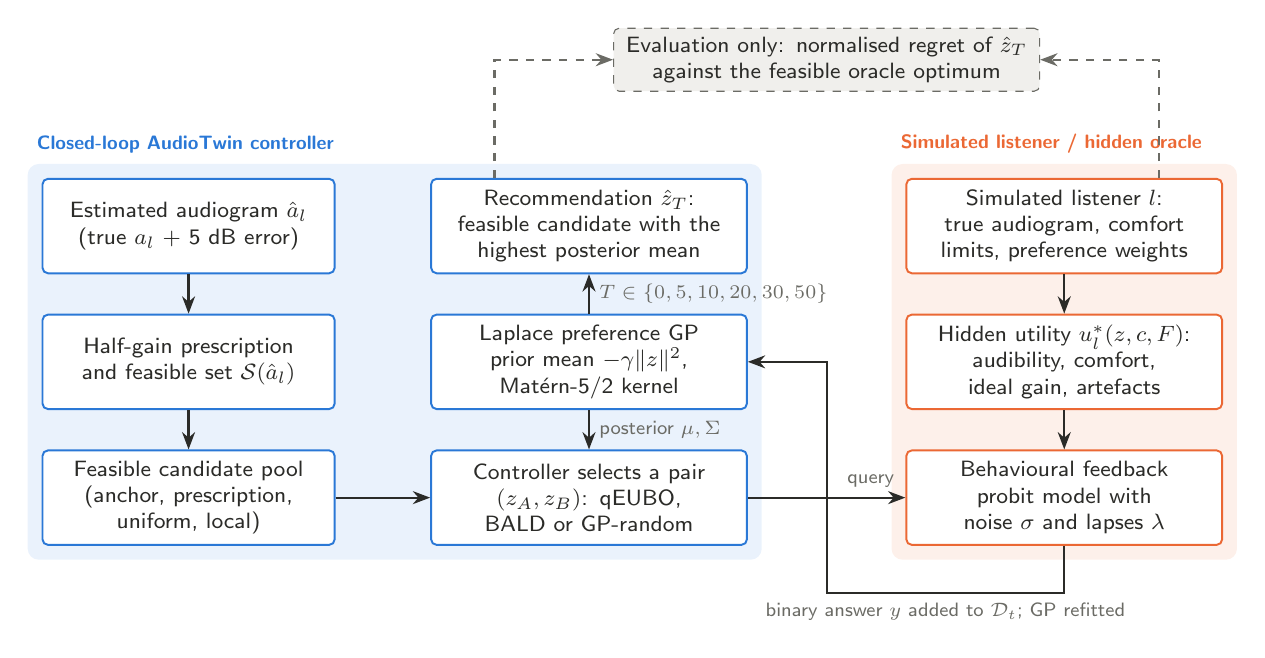
\begin{tikzpicture}[
  font=\footnotesize, text=ink, node distance=5mm and 7mm,
  box/.style={draw=#1, rounded corners=2pt, line width=0.7pt, fill=white, align=center,
              inner sep=3pt, minimum height=12mm, text width=35mm},
  arr/.style={-{Stealth[length=2.2mm]}, line width=0.8pt, draw=ink},
  lab/.style={font=\scriptsize, text=muted, align=center}]

% ---- learner (twin) --------------------------------------------------------------------------
\node[box=learner] (aud) {Estimated audiogram $\hat a_l$\\(true $a_l$ + 5 dB error)};
\node[box=learner, below=of aud] (rx) {Half-gain prescription\\and feasible set $\mathcal S(\hat a_l)$};
\node[box=learner, below=of rx] (pool) {Feasible candidate pool\\(anchor, prescription,\\uniform, local)};
\node[box=learner, right=12mm of pool, text width=38mm] (acq) {Controller selects a pair\\$(z_A, z_B)$: qEUBO,\\BALD or GP-random};
\node[box=learner, above=of acq, text width=38mm] (gp) {Laplace preference GP\\prior mean $-\gamma\|z\|^2$,\\Mat\'ern-5/2 kernel};
\node[box=learner, above=of gp, text width=38mm] (rec) {Recommendation $\hat z_T$:\\feasible candidate with the\\highest posterior mean};

\draw[arr] (aud) -- (rx);
\draw[arr] (rx) -- (pool);
\draw[arr] (pool) -- (acq);
\draw[arr] (gp) -- node[lab, right]{posterior $\mu,\Sigma$} (acq);
\draw[arr] (gp) -- node[lab, right]{$T\in\{0,5,10,20,30,50\}$} (rec);

\begin{scope}[on background layer]
  \node[fill=learnerbg, rounded corners=4pt, inner sep=5pt, fit=(aud)(rx)(pool)(acq)(gp)(rec),
        label={[font=\scriptsize\bfseries, text=learner, anchor=south west]north west:Closed-loop AudioTwin controller}] (L) {};
\end{scope}

% ---- hidden simulated listener --------------------------------------------------------------
\node[box=hidden, right=20mm of acq, text width=38mm] (choice) {Behavioural feedback\\probit model with\\noise $\sigma$ and lapses $\lambda$};
\node[box=hidden, right=20mm of gp, text width=38mm] (util) {Hidden utility $u^*_l(z,c,F)$:\\audibility, comfort,\\ideal gain, artefacts};
\node[box=hidden, right=20mm of rec, text width=38mm] (lis) {Simulated listener $l$:\\true audiogram, comfort\\limits, preference weights};
\draw[arr] (lis) -- (util);
\draw[arr] (util) -- (choice);

\begin{scope}[on background layer]
  \node[fill=hiddenbg, rounded corners=4pt, inner sep=5pt, fit=(lis)(util)(choice),
        label={[font=\scriptsize\bfseries, text=hidden, anchor=south west]north west:Simulated listener / hidden oracle}] (H) {};
\end{scope}

\draw[arr] (acq.east) -- node[lab, above, pos=0.78]{query} (choice.west);
\draw[arr] (choice.south) -- ++(0,-6mm) -| node[lab, pos=0.25, below]{binary answer $y$ added to $\mathcal D_t$; GP refitted} ($(gp.east)+(10mm,0)$) -- (gp.east);

% ---- evaluation only ------------------------------------------------------------------------
\coordinate (rtop) at ($(rec.north)+(-12mm,0)$);
\coordinate (ltop) at ($(lis.north)+(12mm,0)$);
\node[draw=muted, dashed, rounded corners=2pt, fill=evalbg, align=center, text width=52mm, inner sep=3pt,
      minimum height=8mm] (eval) at ($($(rtop)!0.5!(ltop)$)+(0,15mm)$)
      {Evaluation only: normalised regret of $\hat z_T$\\against the feasible oracle optimum};
\draw[arr, dashed, draw=muted] (rtop) |- (eval.west);
\draw[arr, dashed, draw=muted] (ltop) |- (eval.east);
\end{tikzpicture}
\end{document}
